\documentclass[11pt]{scrartcl}
\usepackage[T1]{fontenc}
\usepackage[a4paper, left=3cm, right=2cm, top=2cm, bottom=2cm]{geometry}
\usepackage[activate]{pdfcprot}
\usepackage[ngerman]{babel}
\usepackage[parfill]{parskip}
\usepackage[utf8]{inputenc}
\usepackage[math]{kurier}
\usepackage{amsmath}
\usepackage{amssymb}
\usepackage{xcolor}
\usepackage{epstopdf}
\usepackage{txfonts}
\usepackage{fancyhdr}
\usepackage{graphicx}
\usepackage{prettyref}
\usepackage{hyperref}
\usepackage{eurosym}
\usepackage{setspace}
\usepackage{units}
\usepackage{eso-pic,graphicx}
\usepackage{icomma}
\usepackage{pdfpages}

\definecolor{darkblue}{rgb}{0,0,.5}
\hypersetup{pdftex=true, colorlinks=true, breaklinks=false, linkcolor=black, menucolor=black, pagecolor=black, urlcolor=darkblue}



\setlength{\columnsep}{2cm}


\newcommand{\arcsinh}{\mathrm{arcsinh}}
\newcommand{\asinh}{\mathrm{arcsinh}}
\newcommand{\ergebnis}{\textcolor{red}{\mathrm{Ergebnis}}}
\newcommand{\fehlt}{\textcolor{red}{Hier fehlen noch Inhalte.}}
\newcommand{\betanotice}{\textcolor{red}{Diese Aufgaben sind noch nicht in der Übung kontrolliert worden. Es sind lediglich meine Überlegungen und Lösungsansätze zu den Aufgaben. Es können Fehler enthalten sein!!! Das Dokument wird fortwährend aktualisiert und erst wenn das \textcolor{black}{beta} aus dem Dateinamen verschwindet ist es endgültig.}}
\newcommand{\half}{\frac{1}{2}}
\renewcommand{\d}{\, \mathrm d}
\newcommand{\punkte}{\textcolor{white}{xxxxx}}
\newcommand{\p}{\, \partial}
\newcommand{\dd}[1]{\item[#1] \hfill \\}

\renewcommand{\familydefault}{\sfdefault}
\renewcommand\thesection{}
\renewcommand\thesubsection{}
\renewcommand\thesubsubsection{}


\newcommand{\themodul}{}
\newcommand{\thetutor}{Prof. Förster}
\newcommand{\theuebung}{Formelsammlung - Halbleiter und Nanotechnologie}

\pagestyle{fancy}
\fancyhead[L]{\footnotesize{C. Hansen}}
\chead{\thepage}
\rhead{}
\lfoot{}
\cfoot{}
\rfoot{}

\title{\theuebung{}, \thetutor}


\author{Christoph Hansen \\ {\small \href{mailto:chris@university-material.de}{chris@university-material.de}} }

\date{}


\begin{document}

\maketitle

Dieser Text ist unter dieser \href{http://creativecommons.org/licenses/by-nc-sa/4.0/}{Creative Commons} Lizenz veröffentlicht.

\textcolor{red}{Ich erhebe keinen Anspruch auf Vollständigkeit oder Richtigkeit. Falls ihr Fehler findet oder etwas fehlt, dann meldet euch bitte über den Emailkontakt.}

\tableofcontents


\newpage


Ich habe keine Formeln aus vorigen Übungen inkludiert, da diese recht gut im Skript zusammengefasst sind.



\section{Aus Übung 5}

\begin{align*}
\intertext{Zustandsdichten im k-Raum:} 
D(k)\d k &= \frac{\pi k^2}{\pi^3} \d k 
\intertext{Zustandsdichte im Energieraum:}
D(E) \d E &= \frac{4 \pi \cdot \left( 2m \right)^{3/2)} \cdot \sqrt{E}}{h^3}
\intertext{Dichte der Zustände:}
n &= \int D(E) \d E
\intertext{Wahrscheinlichkeit eines besetzten Elektronenzustandes}
f_h(E) &= \frac{1}{1 + e^{\frac{E - E_F}{kT}}}
\end{align*}



\section{Aus Übung 6}

\begin{align*}
\intertext{Zustandsdichte}
D(E) &= \frac{\d N}{\d E} = \frac{1}{2 \pi^2} \cdot \left( \frac{2m}{\hbar^2} \right)^{\frac{3}{2}} \cdot \sqrt{E} \cdot V
\intertext{Elektronendichte}
n &= \frac{N}{V}
\intertext{Fermienergie}
E_F &= \left( 3 \pi^2 \right)^{\frac{2}{3}} \cdot \frac{\hbar^2}{2m} \cdot n^{\frac{2}{3}} = \frac{E_C - E_V}{2} + \frac{3kT}{4} \cdot \ln\left( \frac{m_h*}{m_e*} \right) \qquad \text{\textcolor{red}{im Skript mit +}}
\intertext{Fermitemperatur}
T_F &= \frac{E_F}{k}
\intertext{Innere Energie von Fermigas}
U &= \frac{3}{5} \cdot N \cdot E_F
\intertext{Teilchendruck}
P &= \frac{\p U}{\p V} = \frac{2}{5} \cdot n \cdot E_F
\intertext{Zustanddichte der Elektronen}
N_C &= 2 \cdot \left( \frac{kT}{2 \pi \hbar} \right)^{3/2} \cdot m*_e^{3/2}
\intertext{Zustanddichte der Löcher}
N_V &= 2 \cdot \left( \frac{kT}{2 \pi \hbar} \right)^{3/2} \cdot m*_h^{3/2}
\intertext{Teilchenenergie (masseabhängig)}
E &= \frac{\hbar^2 \cdot k^2}{2m^*}
\end{align*}


\section{Aus Übung 7}


\begin{align*}
\intertext{Besetzungsdichte bei einem dotierten Halbleiter}
n_d &= N_d \cdot \frac{1}{1 + \half e^{\frac{E - E_F}{kT}}}
\intertext{Zustandsdichte $N_c$}
N_c &= 2 \cdot \left( \frac{2 \pi \cdot m^* \cdot kT}{h^2} \right)^\frac{3}{2}
\intertext{die Elektronenkonzentration dazu ist dann}
n &= N_c \cdot e^{- \frac{E_c - E_F}{kT}}
\intertext{Raumladungsweite bei einem Schottky-Kontakt}
w &= \sqrt{\frac{2 \cdot \epsilon_r \cdot \epsilon_0 \cdot \left( V_{bi} + V_R \right)}{e \cdot N_d}} \qquad \text{Dabei ist  $V_R$ die Gatespannung mit - am Gate}
\intertext{Die Kapazität}
C' &= \frac{C}{A} = \frac{\epsilon_0 \epsilon_r}{w} = \sqrt{\frac{e \cdot N_d \cdot \epsilon_0 \epsilon_r}{\left( V_{bi} + V_R \right)^2}}
\end{align*}


\section{Aus Übung 8}

\begin{align*}
\intertext{Sättigungsstromdichte:}
j_s &= A \cdot T^2 \cdot e^{-e \cdot \frac{\phi_{SB} - \Delta \phi}{kT}}
\intertext{Widerstand:}
R &= \frac{l \phi}{A} = \frac{l}{n \cdot e \cdot \mu \cdot A}
\intertext{Der y-Achsen Abschnitt bei einer Transmissionslinie ist $2R_C$. Es gilt weiter:}
l_0 &= 2 \cdot \frac{R_s}{r_s} \cdot l_T \approx 2 \cdot l_T
\intertext{effektive Kontaktfläche:}
A_{eff} &= A \cdot l_T
\intertext{spezifischer Kontakwiderstand:}
\rho_e &= R_c \cdot A
\intertext{Schottky Barriere}
\phi_{SB} &= V_{bi} + \phi_n
\end{align*}


\section{Aus Übung 9}

\begin{figure}[h]
	\centering
	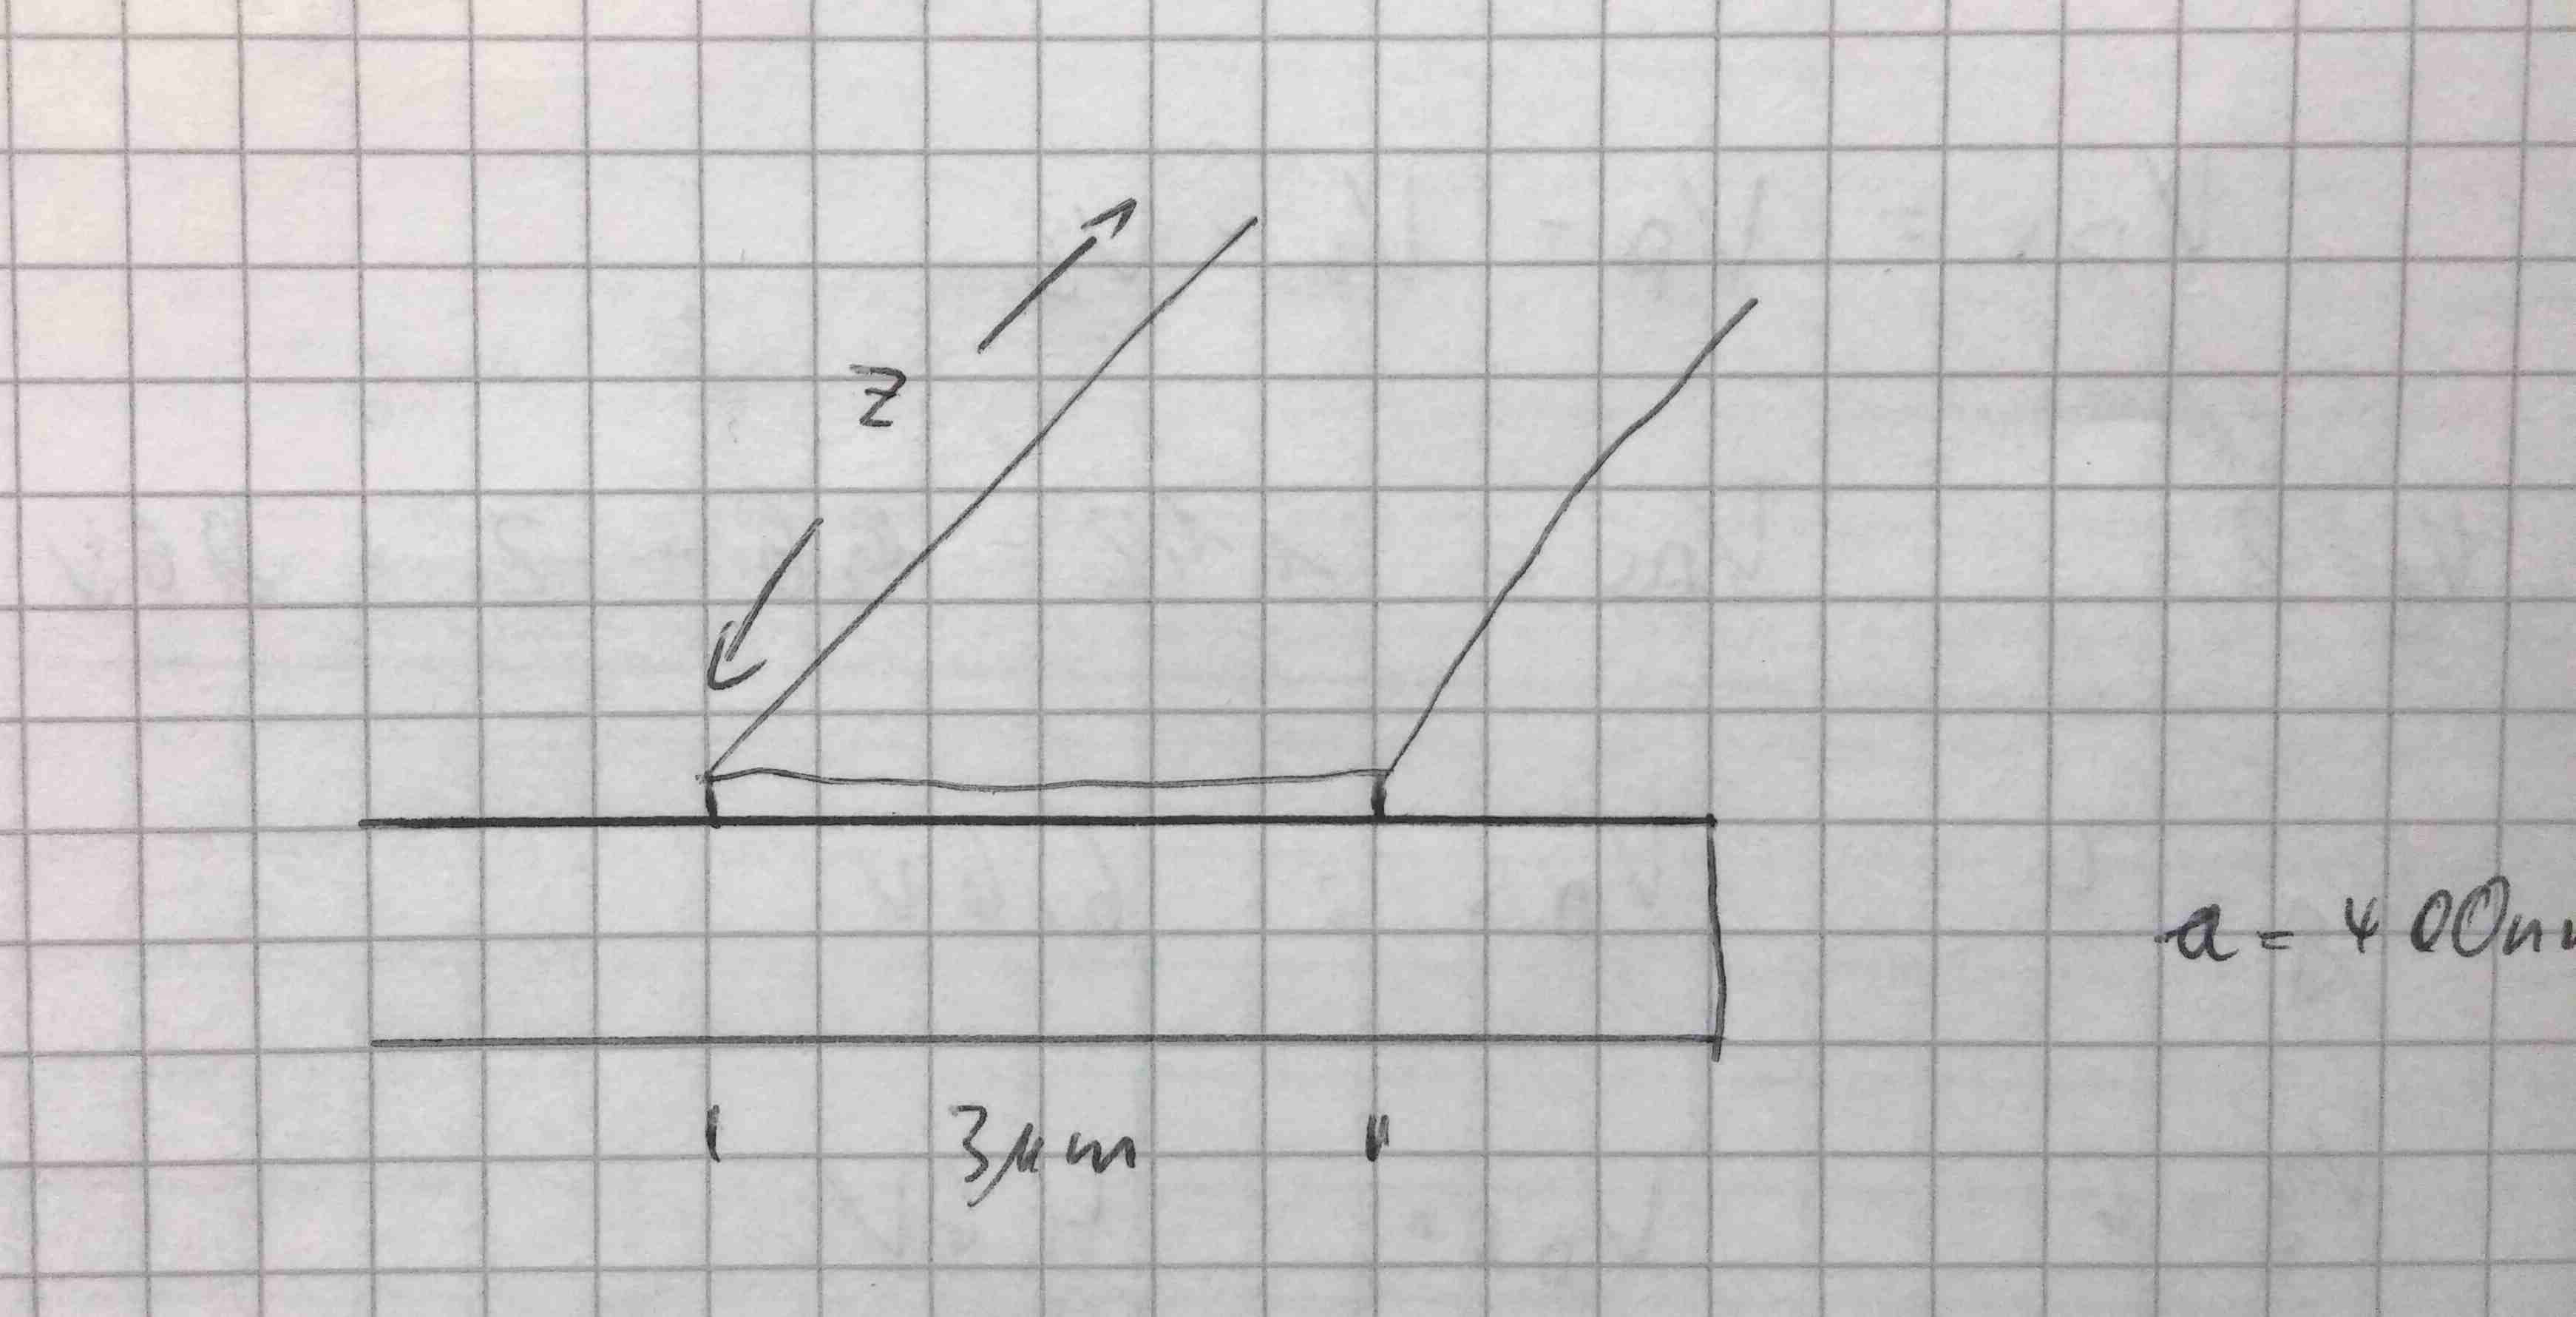
\includegraphics[scale=0.1]{U1_1.jpg}
\end{figure}


\begin{align*}
\intertext{Pinch-Off Spannung}
V_P &= \frac{a^2 \cdot e \cdot N_d}{2 \cdot \epsilon_0 \cdot \epsilon_r}
\intertext{Pinch-Off Strom}
I_P &= \frac{z \cdot \mu \cdot q^2 \cdot N_d^2 \cdot a^3}{6 \cdot \epsilon_0 \epsilon_r \cdot L}
\intertext{Sättigungsstrom}
I_{Sä} &= I_P \cdot \left[ \frac{3 \cdot \left( V_P - V_g - V_{bi} \right)}{V_P} - \frac{2 \cdot \left( V_P^{3/2} - \left( V_g + V_{bi} \right)^{3/2} \right)}{V_P^{3/2}} \right]
\intertext{Drain-Spannung}
V_{DS} &= V_P - V_{bi} - V_g
\intertext{Steilheit}
g_{m} &= I_P \cdot \left[ \frac{-3}{V_P} + \frac{3 \cdot \sqrt{V_g + V_{bi}}}{V_P^{3/2}} \right]
\end{align*}



\section{Transistoren}


\subsection*{Kollektorschaltung}

\begin{figure}[h]
	\centering
	\includegraphics[scale=0.9]{Kollektorschaltung.jpg}
\end{figure}


Spannungsverstärkung kleiner 1, aber sehr hohe Stromverstärkung


\newpage

\subsection*{Emitterschaltung}

\begin{figure}[h]
	\centering
	\includegraphics[scale=0.9]{Emitterschaltung.jpg}
\end{figure}


kleine Stromverstärkung, aber hohe Spannungsverstärkung (keine hohe Frequenzen)



\subsection*{Basisschaltung}

\begin{figure}[h]
	\centering
	\includegraphics[scale=0.9]{Basisschaltung.jpg}
\end{figure}


kann bei hohe Frequenzen als Spannungs und Leistungsverstärker eingesetzt werden.


\subsection*{MOSFET/MESFET}


Der MESFET hat im Gegensatz zum MOSFET einen Metall-Halbleiter Kontakt (Schotky-Kontakt). Dadurch sind bei gleichen Abmessungen höhere Ströme als auch Frequenzen möglich.



\section{Konstanten}

\begin{align*}
e &= \unit[1,6 \cdot 10^{-19}]{V} \\
k &= \unit[1,38 \cdot 10^{-23}]{J/K} \\
\epsilon_0 &= \unit[8,854 \cdot 10^{-12}]{As / Vm} \\
R &= \unit[8,314]{J / mol \ K} \\
m_e &= \unit[9,109 \cdot 10^{-31}]{kg} \\
h &= \unit[6,626 \cdot 10^{-34}]{Js} \qquad \hbar = \frac{h}{2 \pi}
\end{align*}



















\end{document}